\documentclass[pdf]{beamer}
\usepackage[latin1]{inputenc}
\usepackage{multirow}
\usetheme{Warsaw} %Warsaw
\usecolortheme{beetle}

\begin{document}

\title[Differential Expression]{DNA Microarrays\\Differential Expression\\}
\subtitle{BCB 504: Applied Bioinformatics\\}
\author[Matt Settles]{Matt Settles}
\institute{University of Idaho\\ Bioinformatics and Computational Biology Program}
\date{\today}


%% Title page
\begin{frame}[plain]
  \titlepage
\end{frame}


%% Outline
\begin{frame}[plain] 
  \frametitle{Outline}
  \tableofcontents
\end{frame}

\section{Data filtering}

\begin{frame}
  \frametitle{Gene filtering}
  Purpose is to remove probe sets (aka genes) that are likely to be of no use (uninteresting) when modelling the data.
  \begin{description}
  \item[non-specific] Choose genes to remove (or keep) without using any phenotypic variables in the filtering process. Result can then be used with any downstream process without bias.
  \item[specific] Use of phenotypic variables to choose which genes should be kept/removed. Results can be used in a descriptive nature, should not be used for statistical testing.
 \end{description}
\end{frame}

\subsection{Affymetrix PMA Calls}
\begin{frame} 
  \frametitle{Affymetrix Present/Marginal Absent Calls}
  PMA calls - used to determine whether a probe set is reliably detected (Present), not detected (Absent), or marginally detected (Marginal) as being expressed.
  \begin{itemize}
  \item Discrimination score is first calculated for each probe pair.
  \begin{equation}
  (PM-MM)/(PM+MM) - \tau
  \end{equation}
  \item A One-sided Wilcoxon Signed Rank test is used to compare two related samples or repeated measurements on a single sample to assess whether their population mean ranks differ (i.e. it's a paired difference test).
  \item Present absent calls based on resulting p-value
  \begin{itemize}
    \item p-value $<= \alpha_1$ = Present
    \item $\alpha_1 < $ p-value $ < \alpha_2$ = Marginal
    \item $\alpha_2 <= $ p=value = Absent
  \end{itemize}
  \item $\tau = 0.015$, $\alpha_1=0.04$, $\alpha_2=0.06$  
  \end{itemize}
\end{frame}

\begin{frame}[allowframebreaks,fragile]
  \frametitle{Other non-specific filters}
  \begin{description}
  \item [Annotation Based Filtering] Can reduce be a predetermined set of genes (aka entrez ids), by Gene Ontology group, filter based on available annotation data. 
  \item [Duplicate Probe Removal] Probes determined by annotation to be pointing to the same gene are compared, and only the probe with the highest variance value will be retained.
  \item [Variance Based Filtering] Perform numerical cutoff-based filtering (aka IQR). The intention is to remove uninformative probe sets, representing genes that were not expressed at all or no change is occurring. Observations  have shown that unexpressed genes are detected most reliably through their low variability across samples. IQR is robust to outliers, a default cutoff value of 0.5 is motivated by the rule of thumb that in many tissues only 40\% of genes are expressed.
  \end{description}
\end{frame}
%

\section{Differential Expression}
\begin{frame}[allowframebreaks,fragile]
  \frametitle{Approaches}
  \begin{description}
  \item [LIMMA] Linear Models for Microarray Data approach. Limma applies a linear model to the data and uses model contrasts to extract specific comparisons of interest. It then uses multiple testing correction based techniques (FDR, FWER, etc.) for MT corrected p-values. Can also choose a fold change parameter, to ensure that called genes change at least a pre-specified amount. 
  \item [SAM] Significance analysis of Microarrays (SAM) approach. SAM computes a statistic $d_i$ for each gene $i$, measuring the strength of the relationship between gene expression and a response variable. It then uses repeated permutations of the data to determine if the expression of any genes are significantly related to the response. The cutoff for significance is determined by a tuning parameter \textit{delta}, chosen by the user based on the false positive rate. One can also choose a fold change parameter, to ensure that called genes change at least a pre-specified amount.
  \end{description}
\end{frame}

\subsection{SAM}
\begin{frame}
  \frametitle{The SAM plot}
  \begin{center}
  \centering 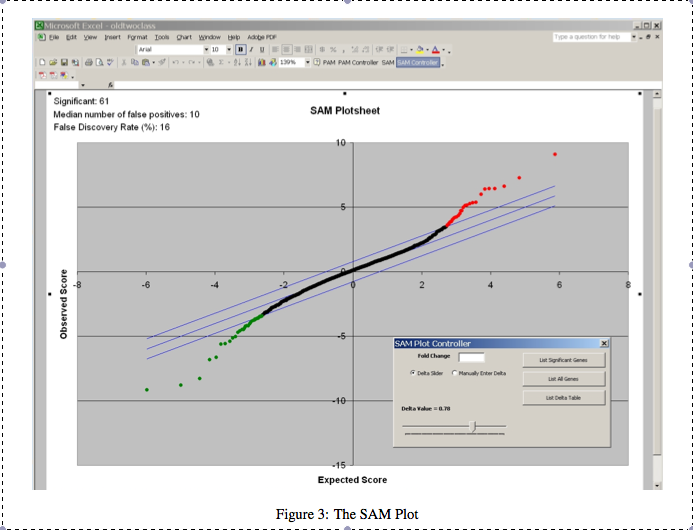
\includegraphics[scale=0.35]{figures/samplot.png}
  \end{center}
\end{frame}

\begin{frame}
  \frametitle{The SAM plot}
  SAM table - gives details about different delta values
  \begin{center}
  \centering 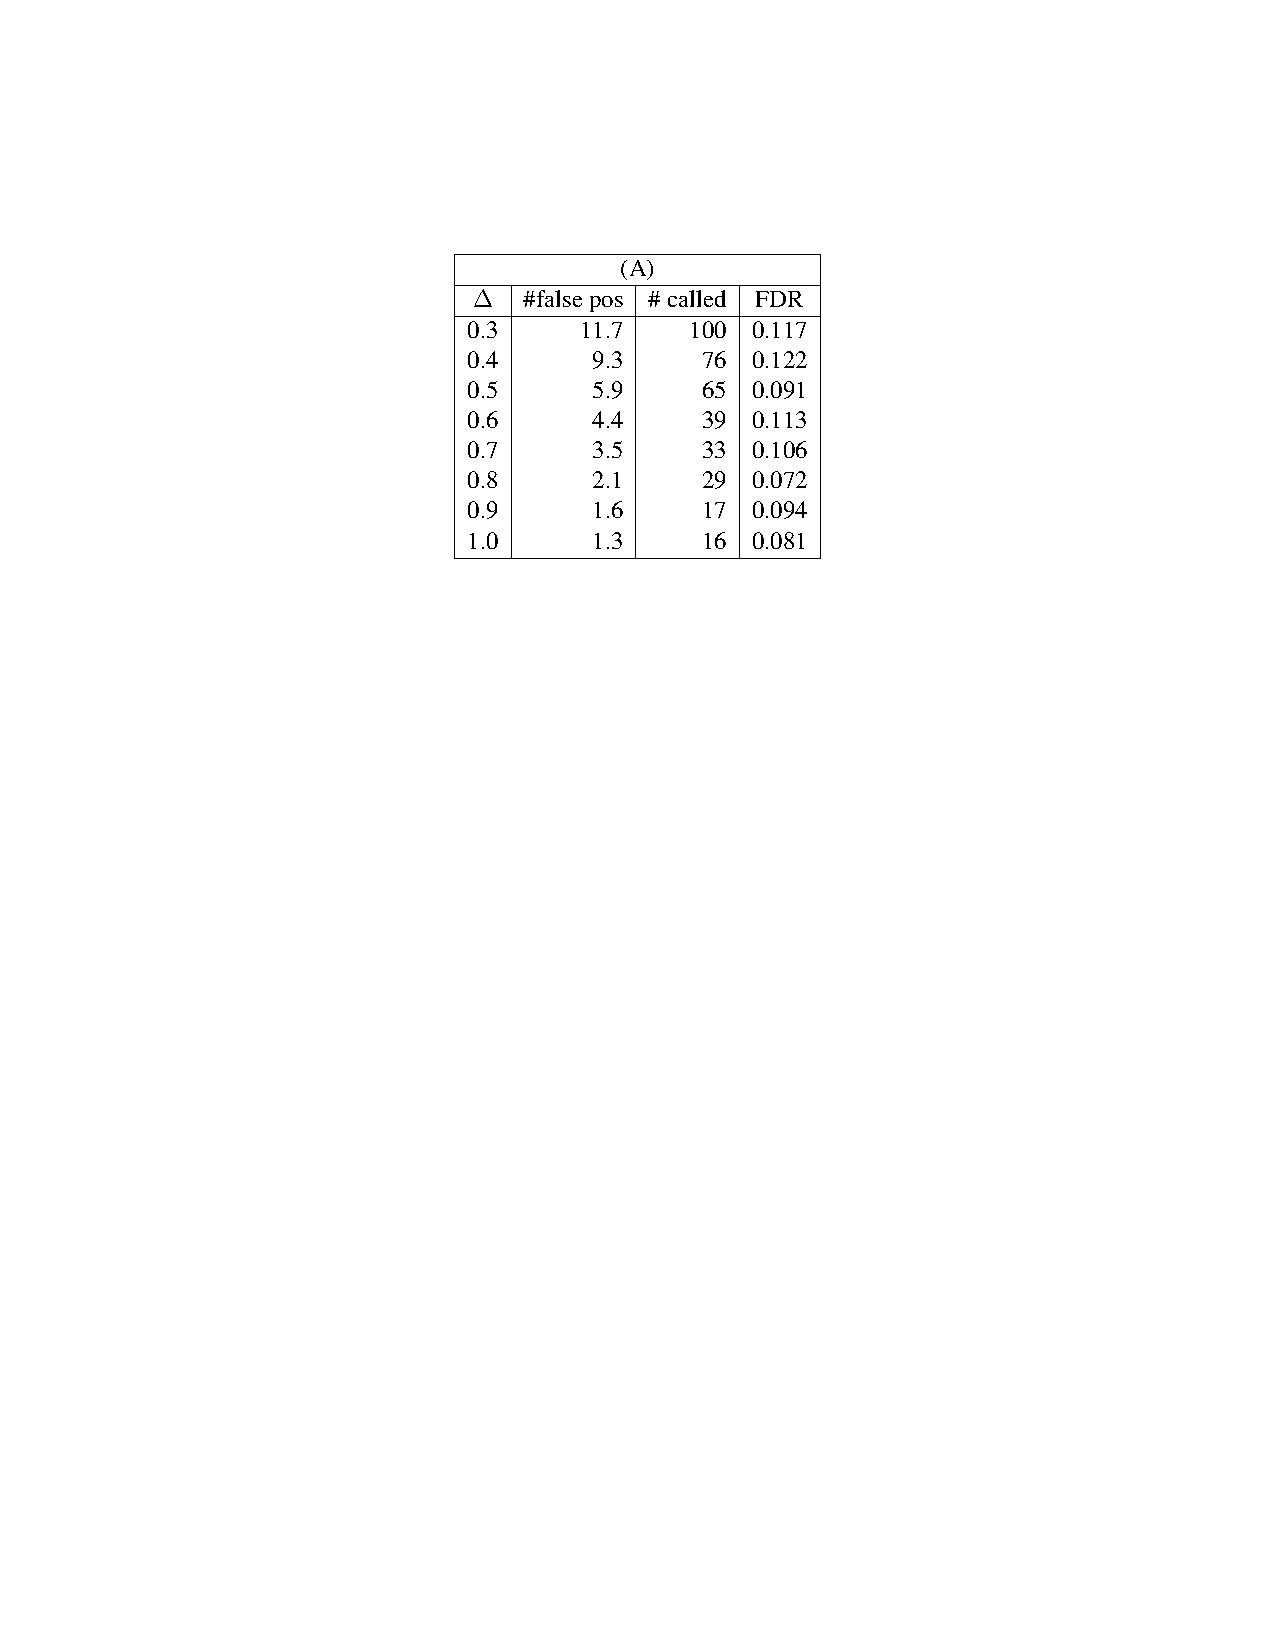
\includegraphics[scale=1.0]{figures/samtable.pdf}
  \end{center}
\end{frame}


\section{Variance Correction}
\begin{frame}
  \frametitle{Variance Corrections}
  \begin{itemize}
  \item When doing statistical test, we estimate the variance for each gene individually. This is fine, \textit{if} we have enough replicates, but with few replicages (say 2-5 per group), these variances are highly variable.
  \item In a moderated statistic, the estimated gene-specific variance $s^2_g$ is replaced by a weighted average of $s^2_g$ and $s^2_0$, which is a global variance estimator obtained from pooling all genes.
  \item This produces an interpolation between the t-test and a fold-change criterion.
  \end{itemize}
Both SAM and LIMMA, perform Variance Correction, SAM bins genes with common fold change, LIMMA performs an empirical Bayes estimate for $s^2_0$.
\end{frame}

\section{Multiple Testing Correction}
\begin{frame}
  \frametitle{Multiple Testing Correction}
  \textbf{Aim:} For a given type I error rate $\alpha$, use a procedure to select a set of "significant" genes that guarantees a type I error rate less than or equal to $\alpha$. 
  \begin{description}
  \item[Bonferonni] Basically multiple raw p-value by the number of tests. \textbf{Unrealistic} given the number of genes tested.
  Many methods available in the bioconductor packages \textit{multtest} and \textit{qvalue}
  \item [Benjimini and Hochberg (BH)] Controls the false discovery rate. Works for independent test statistics and for some types of dependence. Tends to be conservative if many genes are differentially expressed.  
  \item [q-value] the q-value of a gene is defined as the minimal estimated FDR at which it appears significant.
  \end{description}
\end{frame}

% side by side frame
%\begin{frame}
%  \frametitle{The SAM table}
%  \begin{columns}[t] % contents are top vertically aligned
%    \begin{column}[T]{5cm} % each column can also be its own environment
%      \begin{itemize}
%        \item SAM table 
%        \item Can be created from the raw intensities, log intensities, model fitting residuals and other
%        \item Looking for large anomalies
%      \end{itemize}
%     \end{column}
%     \begin{column}[T]{5cm} % alternative top-align that's better for graphics
%       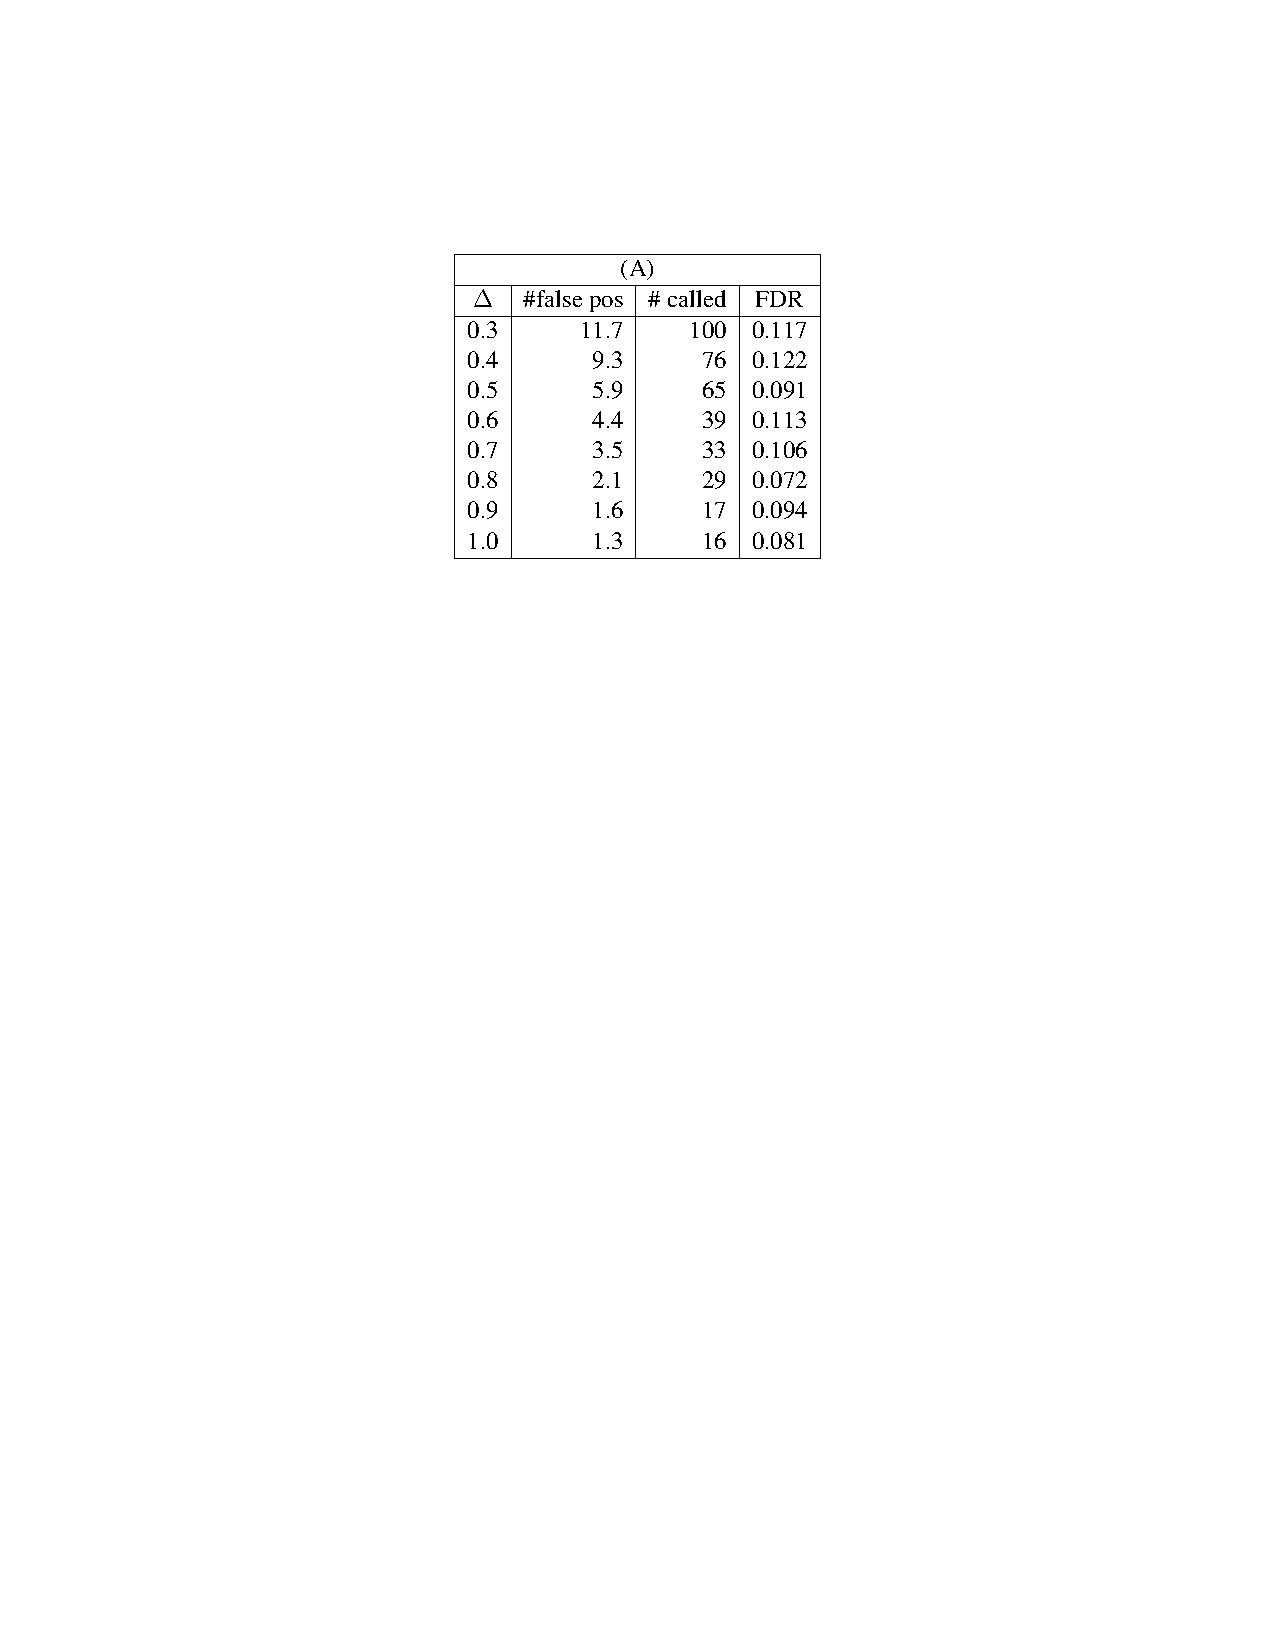
\includegraphics[scale=1.0]{figures/samtable.pdf} 
%     \end{column}
%  \end{columns}
%\end{frame}



%\frame{
%	\begin{description}
%	\item[Description]
%	A data driven approach for the computational and statistical understanding and expertise needed to solve bioinformatics problems that you will likely encounter in your research. 
%	\item[Goals]
%	Following this course the student will be capable of:
%	\begin{itemize} 
%		\item performing their own data analysis project, 
%		\item understanding the technical and statistical tools needed to conduct that analysis
%		\item have the computational ability to do the analysis
%		\item critically review and implement techniques and methods in publications.
%	\end{itemize}
%	\end{description}
%}
%
%\frame{

%\begin{frame}
%    \begin{columns}[c] % the "c" option specifies center vertical alignment
%    \column{.5\textwidth} % column designated by a command
%     Contents of the first column
%    \column{.5\textwidth}
%     Contents split \\ into two lines
%    \end{columns}
%\end{frame}
%
%\begin{frame}
%     \begin{columns}[t] % contents are top vertically aligned
%     \begin{column}[T]{5cm} % each column can also be its own environment
%     Contents of first column \\ split into two lines
%     \end{column}
%     \begin{column}[T]{5cm} % alternative top-align that's better for graphics
% Graphic would go here
%      \end{column}
%     \end{columns}
%\end{frame}
%
%\frame{
%   \begin{block}{This is a Block}
%      This is important information
%   \end{block}
% 
%   \begin{alertblock}{This is an Alert block}
%   This is an important alert
%   \end{alertblock}
% 
%   \begin{exampleblock}{This is an Example block}
%   This is an example 
%   \end{exampleblock}
%}

\end{document}
